\documentclass{beamer}
\usepackage{tikz}
\usepackage{tikzsymbols}
\usepackage{pgfplots}
\usepackage{scalerel}
\usepackage{caption}
\usepackage{subcaption}
\usepackage{mathtools}
\usepackage{hyperref}
\usetikzlibrary{backgrounds}
\usepackage{amsmath}
\usetheme{Boadilla}

%Information to be included in the title page:
\title{\texttt{BisPy}}
\subtitle{un pacchetto Python per il calcolo\\ della massima bisimulazione di grafi diretti.}

\author{Francesco Andreuzzi}
\institute{Università degli Studi di Trieste,\\Dipartimento di Ingegneria e Architettura}
\date{14 Luglio 2021}

\makeatletter
\setbeamertemplate{footline}
{
  \leavevmode%
  \hbox{%
  \begin{beamercolorbox}[wd=.333333\paperwidth,ht=2.25ex,dp=1ex,center]{author in head/foot}%
    \usebeamerfont{author in head/foot}\insertshortauthor%~~\beamer@ifempty{\insertshortinstitute}{}{(\insertshortinstitute)}
  \end{beamercolorbox}%
  \begin{beamercolorbox}[wd=.333333\paperwidth,ht=2.25ex,dp=1ex,center]{title in head/foot}%
    \usebeamerfont{title in head/foot}\insertshorttitle
  \end{beamercolorbox}%
  \begin{beamercolorbox}[wd=.333333\paperwidth,ht=2.25ex,dp=1ex,right]{date in head/foot}%
    \usebeamerfont{date in head/foot}\insertshortdate{}\hspace*{2em}
    \insertframenumber{} / \inserttotalframenumber\hspace*{2ex}
  \end{beamercolorbox}}%
  \vskip0pt%
}
\makeatother

\begin{document}
\beamertemplatenavigationsymbolsempty

{\usebackgroundtemplate{%
    \parbox[c][\paperheight][c]{\paperwidth}{\centering \tikz\node[opacity=0.08] {
\includegraphics[width=8cm,height=8cm]{../imgs/logo.png}};}}
    \begin{frame}
        \maketitle
        {\scriptsize Anno accademico 2020-2021 \hfill Relatore: Prof. Alberto Casagrande}
    \end{frame}
}

% I grafi diretti sono strutture matematiche composte da un insieme V di nodi e da un insieme E di archi. Sono oggetti interessanti
% perchè consentono di creare un modello matematico di sistemi di vario genere (social network, impianti industriali, catene logistiche).
% Per questo motivo lo studio della teoria dei grafi è trasversale rispetto a molti ambiti.
\begin{frame}\frametitle{Grafi diretti}

    \begin{figure}[t]
        \centering
        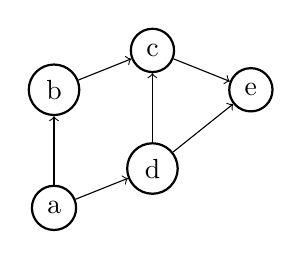
\begin{tikzpicture}[scale=0.5]
            \begin{scope}[every node/.style={circle,thick,draw}]
                \node (a) at (0,0) {a};
                \node (b) at (0,3) {b};
                \node (c) at (2.5,4) {c};
                \node (d) at (2.5,1) {d};
                \node (e) at (5,3) {e};
            \end{scope}

            \begin{scope}
                \path [->] (a) edge node {} (b);
                \path [->] (b) edge node {} (c);
                \path [->] (a) edge node {} (d);
                \path [->] (d) edge node {} (c);
                \path [->] (d) edge node {} (e);
                \path [->] (c) edge node {} (e);
            \end{scope}
            \end{tikzpicture}
    \end{figure}

    \begin{gather*}
        V = \{a,b,c,d,e\}\\
        E = \{\langle a,b\rangle, \langle b,c\rangle, \langle a,d\rangle, \langle c,e\rangle, \langle d,e\rangle\}
    \end{gather*}
\end{frame}

% Per alcune applicazioni può essere utile avere a disposizione una nozione di equivalenza tra nodi. Il mio lavoro di tesi si è
% focalizzato su una possibile definizione di equivalenza, la massima bisimulazione. Due nodi sono bisimili quando preso uno qualsiasi
% dei due, per ogni suo figlio esiste un figlio dell'altro nodo bisimile al primo figlio scelto.
% slide 1, vediamo un esempio. E' chiaro che due pozzi sono bisimili per la definizione.
% slide 2, anche in questo caso è facile verificare la definizione.
% slide 3, è chiaro che aumentando la complessità del grafo diventa impossibile trovare la massima bisimulazione ad occhio.
\begin{frame}\frametitle{Bisimulazione I}
    \begin{block}{Definizione: Bisimulazione}
        \centering
        $a \mathcal{B} b \implies \begin{cases}
            \langle a, a' \rangle \in E \implies \exists b' \mid \langle b, b' \rangle \in E \land a' \mathcal{B} b'\\
            \langle b, b' \rangle \in E \implies \exists a' \mid \langle a, a' \rangle \in E \land b' \mathcal{B} a'
        \end{cases}$
    \end{block}

    \bigskip\bigskip

    \begin{figure}
        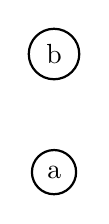
\begin{tikzpicture}[scale=0.5]
            \begin{scope}[every node/.style={circle,thick,draw}]
                \node (a) at (0,0) {a};
                \node (b) at (0,3) {b};
            \end{scope}
            \end{tikzpicture}
    \end{figure}
\end{frame}

\begin{frame}\frametitle{Bisimulazione II}
    \begin{block}{Definizione: Bisimulazione}
        \centering
        $a \mathcal{B} b \implies \begin{cases}
            \langle a, a' \rangle \in E \implies \exists b' \mid \langle b, b' \rangle \in E \land a' \mathcal{B} b'\\
            \langle b, b' \rangle \in E \implies \exists a' \mid \langle a, a' \rangle \in E \land b' \mathcal{B} a'
        \end{cases}$
    \end{block}

    \bigskip\bigskip

    \begin{figure}
        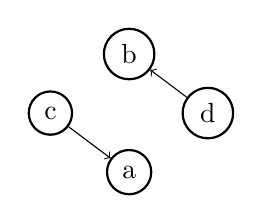
\begin{tikzpicture}[scale=0.5]
            \begin{scope}[every node/.style={circle,thick,draw}]
                \node (a) at (0,0) {a};
                \node (b) at (0,3) {b};
                \node (c) at (-2,1.5) {c};
                \node (d) at (2,1.5) {d};
            \end{scope}

            \begin{scope}
                \path [->] (c) edge node {} (a);
                \path [->] (d) edge node {} (b);
            \end{scope}
            \end{tikzpicture}
    \end{figure}
\end{frame}

\begin{frame}\frametitle{Bisimulazione III}
    \begin{block}{Definizione: Bisimulazione}
        \centering
        $a \mathcal{B} b \implies \begin{cases}
            \langle a, a' \rangle \in E \implies \exists b' \mid \langle b, b' \rangle \in E \land a' \mathcal{B} b'\\
            \langle b, b' \rangle \in E \implies \exists a' \mid \langle a, a' \rangle \in E \land b' \mathcal{B} a'
        \end{cases}$
    \end{block}

    \bigskip\bigskip

    \begin{figure}
        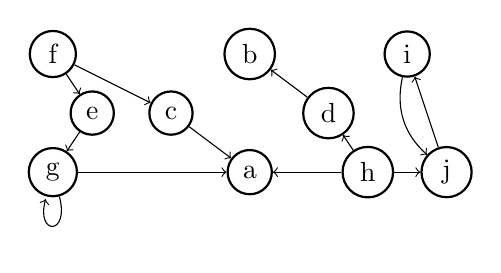
\begin{tikzpicture}[scale=0.5]
            \begin{scope}[every node/.style={circle,thick,draw}]
                \node (a) at (0,0) {a};
                \node (b) at (0,3) {b};
                \node (c) at (-2,1.5) {c};
                \node (d) at (2,1.5) {d};
                \node (e) at (-4,1.5) {e};
                \node (f) at (-5,3) {f};
                \node (g) at (-5,0) {g};
                \node (h) at (3,0) {h};
                \node (i) at (4,3) {i};
                \node (j) at (5,0) {j};
            \end{scope}

            \begin{scope}
                \path [->] (c) edge node {} (a);
                \path [->] (d) edge node {} (b);

                \path [->] (f) edge node {} (c);
                \path [->] (f) edge node {} (e);
                \path [->] (g) edge node {} (a);
                \path [->] (g) edge [loop below] node {} (g);
                \path [->] (e) edge node {} (g);

                \path [->] (h) edge node {} (a);
                \path [->] (h) edge node {} (d);
                \path [->] (i) edge [bend right] node {} (j);
                \path [->] (j) edge node {} (i);
                \path [->] (h) edge node {} (j);
            \end{scope}
            \end{tikzpicture}
    \end{figure}
\end{frame}

\begin{frame}\frametitle{Massima bisimulazione}
    \begin{block}{Definizione: Massima bisimulazione}
        \begin{gather*}
            \mathcal{B}_\mathcal{M} \,\,\,\,\,= \bigcup_{\substack{\mathcal{R} \text{ è una}\\\text{bisimulazione}}} \mathcal{R}.
        \end{gather*}
    \end{block}
    \begin{itemize}
        \item $\mathcal{B}_\mathcal{M}$ è ancora una \emph{bisimulazione};
        \item $\mathcal{B}_\mathcal{M}$ è una \emph{relazione di equivalenza}

        $\implies$ induce un partizionamento su $V$.
    \end{itemize}
\end{frame}

\begin{frame}\frametitle{Algoritmi}
    \begin{itemize}
        \item Algoritmo di Paige-Tarjan;
        \item Algoritmo di Dovier-Piazza-Policriti;
        \item Algoritmo incrementale di Saha.
    \end{itemize}
\end{frame}

\begin{frame}[fragile]\frametitle{BisPy}
    \begin{itemize}
        \item Python 3
        \item Open source (\url{https://github.com/fAndreuzzi/BisPy})
    \end{itemize}


    \begin{example}
        \begin{verbatim}
        import networkx as nx
        from bispy import paige_tarjan

        # creazione del grafo
        graph = nx.balanced_tree(2,3)

        # calcolo della massima bisimulazione
        print(paige_tarjan(graph))

        >>> [(7, 8, 9, 10, 11, 12, 13, 14), (3, 4, 5, 6),
            (1, 2), (0,)]
        \end{verbatim}
    \end{example}
\end{frame}

\begin{frame}\frametitle{Risultati sperimentali I}
    \begin{figure}
        \centering
        \begin{subfigure}[t]{0.49\textwidth}
            \begin{tikzpicture}
                \begin{axis}[
                    axis on top,
                    width=\textwidth,
                    legend style={nodes={scale=0.7, transform shape}, fill=white,opacity=0.8, at={(0,0.68)},anchor=south west, legend columns=1},
                    legend cell align={left},
                    ytick style={draw=none},
                    xtick style={draw=none},
                    xlabel={\texttt{n}},
                    xlabel style={font=\large},
                    ylabel={Secondi},
                    ylabel style={font=\large},
                    xmode=log,
                    ymode=log,
                    grid=major,
                    title={Grafi di Erdős-Rényi}
                ]
                \addplot table[x=x,y=y] {../experiments/time/saha/random/mean_0_0.txt};
                \addlegendentry{Paige-Tarjan}
                \addplot table[x=x,y=y] {../experiments/time/saha/random/mean_0_1.txt};
                \addlegendentry{DPP}
                \addplot table[x=x,y=y] {../experiments/time/saha/random/mean_0_2.txt};
                \addlegendentry{Saha}
            \end{axis}
            \end{tikzpicture}
        \end{subfigure}
        \hfill
        \begin{subfigure}[t]{0.49\textwidth}
            \begin{tikzpicture}
                \begin{axis}[
                    axis on top,
                    width=\textwidth,
                    legend style={nodes={scale=0.7, transform shape}, fill=white,opacity=0.8, at={(0,0.49)},anchor=south west, legend columns=1},
                    legend cell align={left},
                    xlabel={\texttt{depth}},
                    xlabel style={font=\large},
                    ylabel style={font=\large},
                    yminorticks=false,
                    xtick={5.0,6.0,7.0,8.0,9.0,10.0},
                    xticklabels={5,6,7,8,9,10},
                    ymode=log,
                    grid=major,
                    title={Alberi bilanciati}
                ]
                \addplot table[x=x,y=y] {../experiments/time/saha/tree/first/mean_0_0.txt};
                \addlegendentry{Paige-Tarjan}
                \addplot table[x=x,y=y] {../experiments/time/saha/tree/first/mean_0_1.txt};
                \addlegendentry{DPP}
                %\addplot table[x=x,y=y] {experiments/time/saha/tree/second/data1.txt};
                %\addplot table[x=x,y=y] {experiments/time/saha/tree/second/data2.txt};
                \addplot table[x=x,y=y] {../experiments/time/saha/tree/second/data3.txt};
                \addlegendentry{Saha $\Delta v = \hphantom{-}3$}
                \addplot table[x=x,y=y] {../experiments/time/saha/tree/second/datam0.txt};
                \addlegendentry{Saha $\Delta v = \hphantom{-}0$}
                \addplot table[x=x,y=y] {../experiments/time/saha/tree/second/datam1.txt};
                \addlegendentry{Saha $\Delta v = -1$}
                %\addplot table[x=x,y=y] {experiments/time/saha/tree/second/datam2.txt};
                %\addplot table[x=x,y=y] {experiments/time/saha/tree/second/datam3.txt};
                %\addplot table[x=x,y=y] {experiments/time/saha/tree/second/datam4.txt};
                %\addlegendentry{Saha $\Delta v = -4$}
            \end{axis}
            \end{tikzpicture}
        \end{subfigure}
    \end{figure}
\end{frame}

\begin{frame}\frametitle{Risultati sperimentali II}
    \centering
    \begin{figure}
        \begin{subfigure}[t]{\textwidth}
            \begin{tikzpicture}
                \begin{axis}[
                    axis on top,
                    width=\textwidth,
                    height=4.75cm,
                    legend columns=-1,
                    legend style={/tikz/every even column/.append style={column sep=0.5cm}},
                    legend entries={Paige-Tarjan, Dovier-Piazza-Policriti, Saha},
                    legend to name=named5,
                    ytick style={draw=none},
                    xtick style={draw=none},
                    xmajorticks=false,
                    enlargelimits=false,
                    xlabel style={font=\large},
                    ylabel={Secondi},
                    ylabel style={font=\large},
                    ymode=log,
                    grid=major,
                    only marks
                ]
                \addplot+[mark=o,ultra thin,mark options={scale=1}] table[x=x,y=y] {../experiments/time/saha/random/scatter_0_0.txt};
                \addplot+[mark=asterisk,ultra thin,mark options={scale=1}] table[x=x,y=y] {../experiments/time/saha/random/scatter_0_1.txt};
                \addplot+[mark=square,ultra thin,mark options={scale=1}] table[x=x,y=y] {../experiments/time/saha/random/scatter_0_2.txt};
                \addplot+[
                    domain=0:100,
                    samples=100,
                    no marks,
                    sharp plot,
                    color=blue,
                    line width=1pt,
                    solid
                ]
                {0.02367323};
                \addplot+[
                    domain=0:100,
                    samples=100,
                    no marks,
                    sharp plot,
                    color=red,
                    line width=1pt,
                    solid
                ]
                {0.05305607};
                \addplot+[
                    domain=0:100,
                    samples=100,
                    no marks,
                    sharp plot,
                    color=brown,
                    line width=1pt,
                    solid
                ]
                {0.01112568};
            \end{axis}
            \end{tikzpicture}
        \end{subfigure}

        \bigskip

        \begin{subfigure}[t]{\textwidth}
            \begin{tikzpicture}
                \begin{axis}[
                    axis on top,
                    width=\textwidth,
                    height=4.75cm,
                    legend columns=-1,
                    legend style={/tikz/every even column/.append style={column sep=0.5cm}},
                    legend entries={Paige-Tarjan, Dovier-Piazza-Policriti, Saha},
                    legend to name=named5,
                    ytick style={draw=none},
                    xtick style={draw=none},
                    xtick={0.0,20.0,40.0,60.0,80.0,100.0},
                    xticklabels={0,20,40,60,80,100},
                    xlabel style={font=\large},
                    ylabel={Secondi},
                    ylabel style={font=\large},
                    grid=major,
                    enlargelimits=false,
                    ymode=log,
                    only marks
                ]
                \addplot+[mark=o,ultra thin,mark options={scale=1}] table[x=x,y=y] {../experiments/time/saha/tree/scatter_0.txt};
                \addplot+[mark=asterisk,ultra thin,mark options={scale=1}] table[x=x,y=y] {../experiments/time/saha/tree/scatter_1.txt};
                \addplot+[mark=square,ultra thin,mark options={scale=1}] table[x=x,y=y] {../experiments/time/saha/tree/scatter_2.txt};
                \begin{scope}[on background layer]
                    \fill[green,opacity=0.4] ({rel axis cs:0,0}) rectangle ({rel axis cs:0.04,1});
                    \fill[cyan,opacity=0.4] ({rel axis cs:0.04,0}) rectangle ({rel axis cs:0.09,1});
                    \fill[lightgray,opacity=0.4] ({rel axis cs:0.09,0}) rectangle ({rel axis cs:0.14,1});
                    \fill[magenta,opacity=0.4] ({rel axis cs:0.14,0}) rectangle ({rel axis cs:0.26,1});
                    \fill[lime,opacity=0.4] ({rel axis cs:0.26,0}) rectangle ({rel axis cs:0.68,1});
                    \fill[orange,opacity=0.4] ({rel axis cs:0.68,0}) rectangle ({rel axis cs:0.81,1});
                    \fill[pink,opacity=0.4] ({rel axis cs:0.81,0}) rectangle ({rel axis cs:0.89,1});
                    \fill[teal,opacity=0.4] ({rel axis cs:0.89,0}) rectangle ({rel axis cs:0.92,1});
                    \fill[teal,opacity=0.4] ({rel axis cs:0.92,0}) rectangle ({rel axis cs:1,1});
                \end{scope}
            \end{axis}
            \end{tikzpicture}
        \end{subfigure}
    \end{figure}
    \ref*{named5}
\end{frame}

\begin{frame}\frametitle{Conclusioni e sviluppi futuri}
    \begin{itemize}
        \item Incremental delete: ricalcolo incrementale della massima bisimulazione dopo la \textbf{rimozione} di un arco;
        \item Massima bisimulazione con \emph{labeled edges};
        \item Migliore integrazione con altre librerie (\texttt{NetworkX});
        \item Riscrittura in \texttt{Cython} di parti critiche del codice.
    \end{itemize}

    \begin{block}{Definizione: Bisimulazione con \emph{labeled edges}}
        \begin{gather*}
            a \mathcal{B} b \implies
            \begin{cases}
                \langle a, a' \rangle^\ell \in E \implies \exists b' \mid \langle b, b' \rangle^\ell \in E \land a' \mathcal{B} b'\\
                \langle b, b' \rangle^\ell \in E \implies \exists a' \mid \langle a, a' \rangle^\ell \in E \land b' \mathcal{B} a'
            \end{cases}
        \end{gather*}
    \end{block}
\end{frame}

\begin{frame}
    Grazie per l'attenzione
\end{frame}

\begin{frame}\frametitle{Risultati sperimentali: Paige-Tarjan, Dovier-Piazza-Policriti}
    \begin{figure}[b!]
        \centering
        \begin{subfigure}[t]{0.49\textwidth}
            \begin{tikzpicture}
                \begin{axis}[
                    axis on top,
                    width=\textwidth,
                    ytick style={draw=none},
                    xtick style={draw=none},
                    legend columns=-1,
                    legend style={/tikz/every even column/.append style={column sep=0.5cm}},
                    legend entries={Paige-Tarjan, Dovier-Piazza-Policriti},
                    legend to name=named2,
                    xmode=log,
                    ymode=log,
                    ylabel={Secondi},
                    grid=major,
                    title={Alberi bilanciati}
                ]
                \addplot table[x=x,y=y] {../experiments/time/tree/pta.txt};
                \addplot table[x=x,y=y] {../experiments/time/tree/fba.txt};
                \end{axis}
            \end{tikzpicture}
        \end{subfigure}
        \hfill
        \begin{subfigure}[t]{0.49\textwidth}
            \begin{tikzpicture}
                \begin{axis}[
                    axis on top,
                    width=\textwidth,
                    ytick style={draw=none},
                    xtick style={draw=none},
                    grid=major,
                    xmode=log,
                    ymode=log,
                    title={Automi di Hopcroft}
                ]
                \addplot table[x=x,y=y] {../experiments/time/hopcroft/pta.txt};
                \addplot table[x=x,y=y] {../experiments/time/hopcroft/fba.txt};
                \end{axis}
            \end{tikzpicture}
        \end{subfigure}
        \ref*{named2}
    \end{figure}
\end{frame}

\end{document}
